\chapter{Analysis}

The analysis section of the thesis starts with demonstration of interactive
proofs with goal to build up intuition behind interactive proofs \cite{Goldwasser1989,youtubeMOOCLecture1}.
This section explains how Alice attempts to prove to Bob that she knows an
algorithm, with which she computes some pair (N, y), such that this pair is
part of the quadratic residue language QR. Specifically, Alice needs to
convince Bob that there exists an x such that y equals x squared modulo N,
effectively placing the pair (N, y) within the QR language, which includes all
pairs where y is a quadratic residue of N.

The analysis section continues by highlighting a practical limitation of
interactive proofs in real world cryptography. It notes that for Alice to
prove something to multiple parties, she would need to engage in separate
interactions with each one. This approach is not scalable and becomes
impractical for widespread verification needs. However, the thesis introduces
the Fiat-Shamir transform \cite{Fiat}, a significant breakthrough that addresses this
issue. This transform allows for converting the interactive proof into a
non-interactive format by processing the interaction transcript, making the
proof more practical and scalable for real-world cryptographic applications.

While in theory any NP statement \cite{goldreich1991proofs} can be proven using
interactive proofs, practical implementation requires specific definition and
encoding of the statement. There are two main models of general computation,
those are circuits and turing machines. To trace the computation of a turing
machine, the representation needs to somehow handle memory and thus would accrue
more complexity than if a circuit is used. To represent a statement as a
circuit, an arithmetic circuit, a computation model composed of addition and
multiplication operations, is used. This circuit encodes the statement into a
form suitable for "zk-ifying", enabling the application of interactive proofs
to a broader range of practical scenarios.

The analysis section then explores SNARKs (Succinct Non-interactive ARguments
of Knowledge), which are most commonly used ZKP system today. They are succinct,
meaning that the size of the proof is small and have a relatively fast verification
time.

The final part of the analysis examines how ZKP systems such as SNARKs enable
the creation of a stealth address scheme that upholds privacy and security.
This section assesses how these systems fulfill the necessary properties for a
stealth address scheme, focusing on their ability to ensure transaction
confidentiality while maintaining the anonymity of the recipient's identity.

\section{Proof of quadratic residuosity}

This first part focuses on demonstrating an interactive proof where Alice aims
to prove to Bob that she knows an algorithm, which computes some pair (N, y),
such that this pair is part of the quadratic residue language QR \cite{Goldwasser1989}.
QR is defined as:

\[QR = \lbrace(N, y): \exists x, y \equiv x^2 \pmod{N}\rbrace\]

\begin{figure}[h!]
    \centering
    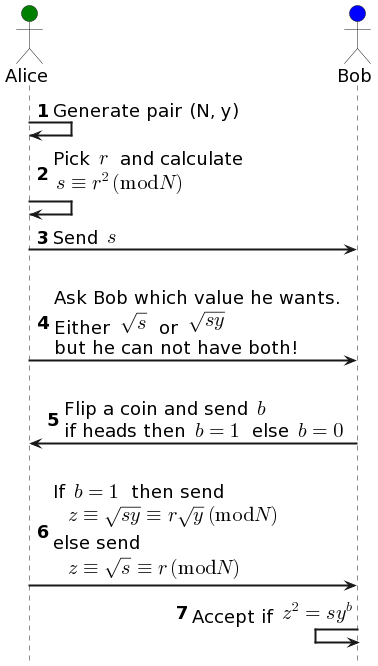
\includegraphics[scale=0.6]{assets/images/qr_ip.png}
    \caption{Interactive proof of language QR}
    \label{fig:qr_ip}
    \vspace{0.5cm}
\end{figure}

\begin{enumerate}
    \item Alice generates pair (N, y)
    \item Alice picks a random $r$ such that $1 \leq r \leq N$ and $\gcd(r, N) = 1$
          and calculates $s \equiv r^2 \pmod{N}$
    \item Alice sends Bob $s$
    \item Alice asks Bob which value he wants. Either $\sqrt{s}$ or $\sqrt{sy}$, but he can not have both!
    \item Bob flips a coin and sends $b$ such that if coin landed on heads $b = 1$ else $b = 0$
    \item If $b = 1$ Alice sends to Bob $z \equiv \sqrt{sy} \equiv r \sqrt{y} \pmod{N}$ else she sends $z \equiv \sqrt{s} \equiv r \pmod{N}$
    \item Bob accepts if $z^2 = sy^b$
\end{enumerate}

If Alice was a cheating prover, and she didn't have the algorithm for
generating pairs from QR, then the probability that Bob's coin toss favors
Alice is one half. With one half probability Bob would ask cheating prover
Alice to give him the equation she can not solve, because if the prover is
cheating, she can not find the $\sqrt{s}$ and $\sqrt{sy}$. If she could,
that would mean that she is not cheating.

If the Alice's claim is true, Bob will accept. If Alice is not honest, and
cheats, all provers will not accept with probability $P(Accept) = 0.5$.
But this probability may not be satisfying enough. To make the probability
that Alice is cheating smaller, Bob and Alice can start the interaction once
again. This would lead to $P(Accept) = (0.5)^2$. They can redo the process
as many times as they wish, resulting in $P(Accept) = (0.5)^k$ where $k$
is how many different interactions they performed.

Thanks to the randomness of the coin toss, there are $2^k$ possibilities how
the interaction can go. Since Alice can't reliably predict what the random
coin toss will yield, she must be ready to provide both equations. Thus Bob is
convinced, that Alice isn't cheating, with probability $P(Accept) = (0.5)^k$,
and can accept the proof.

\section{Non-interactive proofs}

Interactive proofs require Alice to engage in a unique interaction with each
individual verifier, which is not scalable or feasible for widespread
application. Many ZKP protocols only require from the verifier a random input
(for instance, a coin toss). Protocols, in which the verifier's role is
generating some randomness and making it public are called public coin protocols \cite{Babai1988,Goldwasser1986}.
The paper "How To Prove Yourself: Practical Solutions to Identification and
Signature Problems"\cite{Fiat} by Fiat and Shamir demonstrates how these
interactive public coin protocols can be efficiently transformed into
non-interactive ones, offering a more scalable and practical solution for ZKPs.

To transform a interactive public coin protocol into a non-interactive,
Alice uses a random oracle which can provide a random coin toss based on some
input. In practice the source of randomness of the random oracle is a
cryptographic hash function, such as SHA256. Instead of sending messages back
and forth between Alice and Bob, Alice provides to Bob a transformed
transcript of the interaction. Since Bob's role in this interaction would only
be generating random coin toss, Alice can in advance query the random oracle
for this random value, and supply the message as an input to the query. The
transcript string would look like this $(msg1, query(msg1), msg2, ...)$, where $query$ is
the output from random oracle. This string and the public input of the proof
can then be published and anybody, not just Bob, can validate this proof
on their own.

In scenario when Alice sends only two messages and requires one random coin toss
from Bob,
\begin{figure}[h]
    \centering
    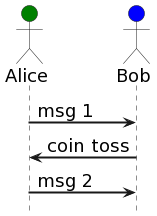
\includegraphics[scale=0.6]{assets/images/interactive_coin.png}
    \caption{Interactive public coin proof}
    \label{fig:interactive_coin}
    \vspace{0.5cm}
\end{figure}
Bob at the end can compute the validity of the proof from Alice with
$validate(public\:input\:x,\:msg1,\:coin\:toss,\:msg2) = accept/reject$

Then after applying Fiat-Shamir transform, Alice only sends one message with
the transcript string,
\begin{figure}[h]
    \centering
    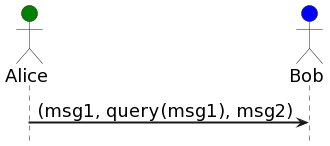
\includegraphics[scale=0.6]{assets/images/non_interactive_coin.png}
    \caption{Non-interactive public coin proof}
    \label{fig:non_interactive_coin}
    \vspace{0.5cm}
\end{figure}
and Bob can compute the validity of the proof like this
$validate(public\:input\:x,\:msg1,\:query(msg1),\:msg2) = accept/reject$.

\section{Arithmetic circuit}

The computation model used to create ZKPs is an arithmetic circuit in a
finite field $\mathbb{F}_p$. The arithmetic circuit is a function which takes
$n$ elements from field $\mathbb{F}_p$ and returns one element from that field.

\[AC: \mathbb{F}^n \rightarrow F \]

The $AC$ can be represented as a directed acyclic graph, or a polynomial. For
example, polynomial $x_1x_2 + (x_2 + x_3)^2$ represents the same circuit as this
directed acyclic graph

\begin{figure}[h]
    \centering
    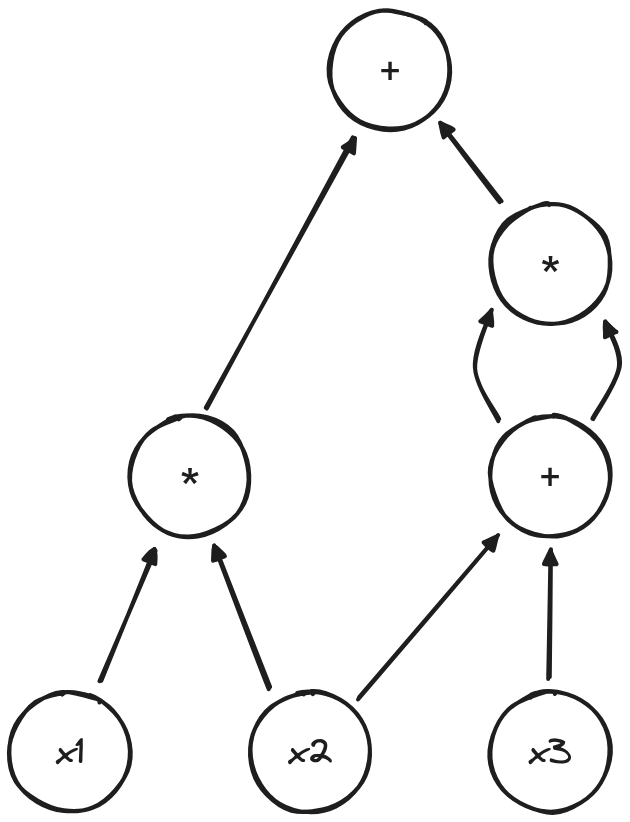
\includegraphics[scale=0.25]{assets/images/dag_example.png}
    \caption{Graph representation of arithmetic circuit}
    \label{fig:dag_example}
    \vspace{0.5cm}
\end{figure}

Another representation of a arithmetic circuits is called a Rank 1 Constraint
System (R1CS). R1CS is a system of equations of a form $\alpha \times \beta = \gamma$,
where $\alpha, \beta, \gamma$ are affine combinations of variables $w$ and $x$,
where $w$ is a witness (private inputs) and $x$ is a public inputs.

These are some examples of R1CS equations:
\begin{displaymath}
    \begin{array}{l}
        (w_1 + x_3) \times (w_2 - x_1 + 1) = w_3 \\
        w_1 \times w_1 = x_1                     \\
        w_1 \times x_2 = w_3
    \end{array}
\end{displaymath}

And here is an example of a invalid R1CS equations, because they are not linear
combinations of variables $w$ and $x$:

\begin{displaymath}
    \begin{array}{l}
        w_1 \times x_3 \times w_2 = w_3 \\
        w_1 \times w_1 \times w_1 = x_1 \\
        w_1 \times x_2 + w_3 = w_4 \times w_5
    \end{array}
\end{displaymath}

To constrain the operation $w_1^3 = x_1$ in R1CS, there must be two equations, with
a new intermediary variable $w_2$:

\begin{displaymath}
    \begin{array}{l}
        w_1 \times w_1 = w_2 \\
        w_1 \times w_2 = x_1
    \end{array}
\end{displaymath}

\section{SNARKs}

After defining an arithmetic circuit, it can be transformed into a SNARK,
a Succinct Non-interactive ARgument of Knowledge. The succint part means that
the size of the proof must be sublinear in size of witness (when talking about
strong succinctness, the proof size is logarithmic in size of circuit), and
the verification must be sublinear in size of circuit and linear in size of
public input (when talking about strong efficiency, the verification time is
logarithmic in size of circuit and linear in size of public input).
A SNARK is a tripple of algorithms $(Setup, Prove, Verify)$.

\subsection{Setup}

The $Setup$ takes
the arithmetic circuit $C(x, w) \rightarrow \mathbb{F}$, where $x$ is a public
input (from $\mathbb{F}^n$) and $w$ is a witness (from $\mathbb{F}^m$), and
is preprocessed, which creates public parameters $pp$ (prover's parameters)
and $vp$ (verifier's parameters). This setup process is what enables the
proof to be logarithmic in size of circuit. It is a summary of the circuit,
so the verifier does not need to know the whole circuit, just the summary.

This setup procedure has 3 types:

\begin{itemize}
    \item Trusted setup: the setup is of form $Setup(C, r) \rightarrow (pp, vp)$,
          where $r$ is a random value. The random value must be destroyed after
          the setup, because if it is not, the prover can use it to prove a false
          statement.
    \item Universal trusted setup: the setup is split into two parts. The first
          part takes only $r$ and creates $gp$ (global parameters). This part
          is ran once and the $r$ must be destroyed, due to the same reason as
          in trusted setup. The second part takes $gp$ and $C$ and creates
          $pp$ and $vp$. This part can be ran for any circuit $C$.
    \item Transparent setup: the setup is of form $Setup(C) \rightarrow (pp, vp)$,
          where $C$ is a circuit. This setup does not require any random value,
          hence anyone can verify that the setup is valid.
\end{itemize}

\subsection{Prove and Verify}

The $Prove$ algorithm takes the prover's parameters $pp$, public input $x$,
witness $w$ and creates a proof $\pi$ which proves that $C(x, w) = 0$.
The $Verify$ algorithm takes the verifier's parameters $vp$, public input $x$ and
proof $\pi$ and returns $accept/reject$. These algorithms combine two
cryptographic primitives, a functional commitment scheme and an interactive
oracle proof, in order create and verify the proof.

Functional commitment scheme is a cryptographic primitive, which allows the
prover to commit to a function $f$ and the verifier can query the commitment and
prover must provide the evaluation of the function $f$ at the queried point,
and a proof that the evaluation is correct.

The interactive oracle proof begins with instantiating $vp$ in the setup phase, such that
$vp = (comm_{f1}, comm_{f2}, \dots, comm_{fn})$, where $comm_{fi}$ is a
functional commitment for a function $f_i$. Verifier can interactively query
any of the commitments and prover must provide the evaluation of the function
$f_i$ at the queried point, and a proof that the evaluation is correct.
Then during the interaction prover and verifier exchange additional function
commitments $comm_{f1}, comm_{f2}, \dots, comm_{fm}$, and random values $r_1, r_2, \dots, r_m$.
At the end verifier computes:

\[ Verify^{comm_{f1}, comm_{f2}, \dots, comm_{fm}, \ldots, comm_{fn}}(x, r_1, r_2, \dots, r_m) = accept/reject \]

The $Verify$ algorithm computes if the proof is valid, based on queried
function commitments from $vp$, and the function commitments which were
exchanged during the interaction. Verifier checks if evaluations
of committed polynomials are equal to evaluations of the polynomials, which
verifier can compute from the public input $x$, proving that the prover's
polynomials are equal to the verifier's polynomials. Elaboration why evaluation
at random point is enough to prove that two polynomials are equal can be found
Appendix \ref{appendix:zero_test}.

To make this process non-interactive, the Fiat-Shamir transform is applied on
the random values $r_1, r_2, \dots, r_m$. So the proof $\pi$ is a string of
\[ (comm_{f1}, FS(r_1), comm_{f2}, FS(r_2), \dots, comm_{fm}, FS(r_m)) \]
Verifier than computes $Verify(vp, x, \pi) = accept/reject$, where $\pi$ is
a transcript of the interaction between prover and Fiat-Shamir supplied random
values.

\section{Stealth addresses}

Ethereum is a public blockchain, where all transactions are visible to anyone,
and all addresses are visible to anyone. This is a problem for privacy, because
if someone knows your address, they can see all your transactions.

One solution to this problem is to generate a new address for every transaction.
However, if somebody wants to send you some funds, they need to wait for you to
generate a new address and send it to them. Which quickly becomes impractical.

The concept of stealth addresses was introduced in 2014 by Peter Todd \cite{ToddStealthAddresses}.
It enables senders to send funds to a recipient without leaking the recipient's
identity to the public. Only the recipient can then prove that they own the stealth
address, and can spend the funds.

For a recipient to receive funds, they need to publish a meta stealth address,
from which senders can generate a new stealth address. This new stealth address
can not be linked to the meta stealth address, and thus the recipient's identity
is protected. Additionally, senders must publish some information, which allows
the recipient to derive the private key for the stealth address.

ZKPs can be used to prove that the recipient owns the stealth address, and
thus can spend the funds. The proof can be sent from any address, but only
the recipient can generate it, because only he knows the private data
that is required to generate the proof. The zero knowledge property of the
proof ensures that the recipient's identity is not revealed.


